% mn2esample.tex
%
% v2.1 released 22nd May 2002 (G. Hutton)
%
% The mnsample.tex file has been amended to highlight
% the proper use of LaTeX2e code with the class file
% and using natbib cross-referencing. These changes
% do not reflect the original paper by A. V. Raveendran.
%
% Previous versions of this sample document were
% compatible with the LaTeX 2.09 style file mn.sty
% v1.2 released 5th September 1994 (M. Reed)
% v1.1 released 18th July 1994
% v1.0 released 28th January 1994


\documentclass[useAMS,usenatbib]{mn2e}
\usepackage{graphicx}

% If your system does not have the AMS fonts version 2.0 installed, then
% remove the useAMS option.
%
% useAMS allows you to obtain upright Greek characters.
% e.g. \umu, \upi etc.  See the section on "Upright Greek characters" in
% this guide for further information.
%
% If you are using AMS 2.0 fonts, bold math letters/symbols are available
% at a larger range of sizes for NFSS release 1 and 2 (using \boldmath or
% preferably \bmath).
%
% The usenatbib command allows the use of Patrick Daly's natbib.sty for
% cross-referencing.
%
% If you wish to typeset the paper in Times font (if you do not have the
% PostScript Type 1 Computer Modern fonts you will need to do this to get
% smoother fonts in a PDF file) then uncomment the next line
% \usepackage{Times}

%%%%% AUTHORS - PLACE YOUR OWN MACROS HERE %%%%%


%%%%%%%%%%%%%%%%%%%%%%%%%%%%%%%%%%%%%%%%%%%%%%%%

\title[Disc stuff]{Disc stuff}
\author[Tom  Douglas, Paola Caselli, Et al.]{Tom Douglas$^{1}$\thanks{E-mail:
pytd@leeds.ac.uk}, Paola Caselli$^{1}$\\
$^{1}$School of Physics and Astronomy, University of Leeds, Leeds LS2 9JT, UK}
\begin{document}

\date{In original form 2012}

\pagerange{\pageref{firstpage}--\pageref{lastpage}} \pubyear{2002}

\maketitle

\label{firstpage}

\begin{abstract}
Abstract here
\end{abstract}

\begin{keywords}
circumstellar matter -- infrared: stars.
\end{keywords}

\section{Introduction}

1. description of what has been done so far on the modelling and radiative transfer of disks (this includes also more evolved disks -- Visser et al., Walsh et al., Aikawa et al. ..)
2. focus on the young disks (work done by Machida et al., Dapp, Basu \& Kunz 2012, .. for their formation; work by Boley et al. on the physical evolution ; Ilee et al. for chemistry) 
3. previous attempts to observe these young disks: (a) simulations (Cossins et al. 2010); (b) observations: Fuente et al. 2010 (AB Aur); Jorgensen \& van Dishoeck (H$_2^{18}$O and the HDO/H2O ratio); Pineda et al. (2012); other papers talking about "hot corinos" (Bottinelli et al. ....)

\section{Description of the Model}

-describe the envelope structure (pre-stellar core)
Keto \& Caselli model (2010), disc is embedded in an infalling pre-stellar core, with densities temperatures and velocities given by the model of the collapse of a 10 solar mass Bonnor-Ebert sphere and providing similar line profiles to the pre-stellar core L1544 as described by Keto \& Caselli (2010), with some slight modification due to the addition of Oxygen lines (keto et al 2012 in prep). This prestellar core model extends from 80$\,$au out to 10,000$\,$au. The model is 1D spherically symmetric model with inward motions (see figure).

\begin{figure}
 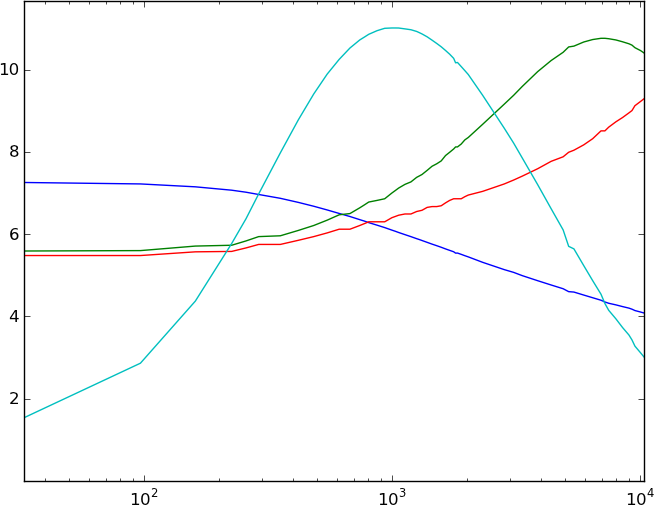
\includegraphics[width=84mm]{Figures/model/L1544model_used.png}

 \caption{envelope model with temp and dust temp (red, green) in kelvin, log number density (blue) in cm$^{-3}$ and inward velocity$\times$100 (cyan) in m$\,$s$^{-1}$}
\end{figure}

\begin{figure*}
 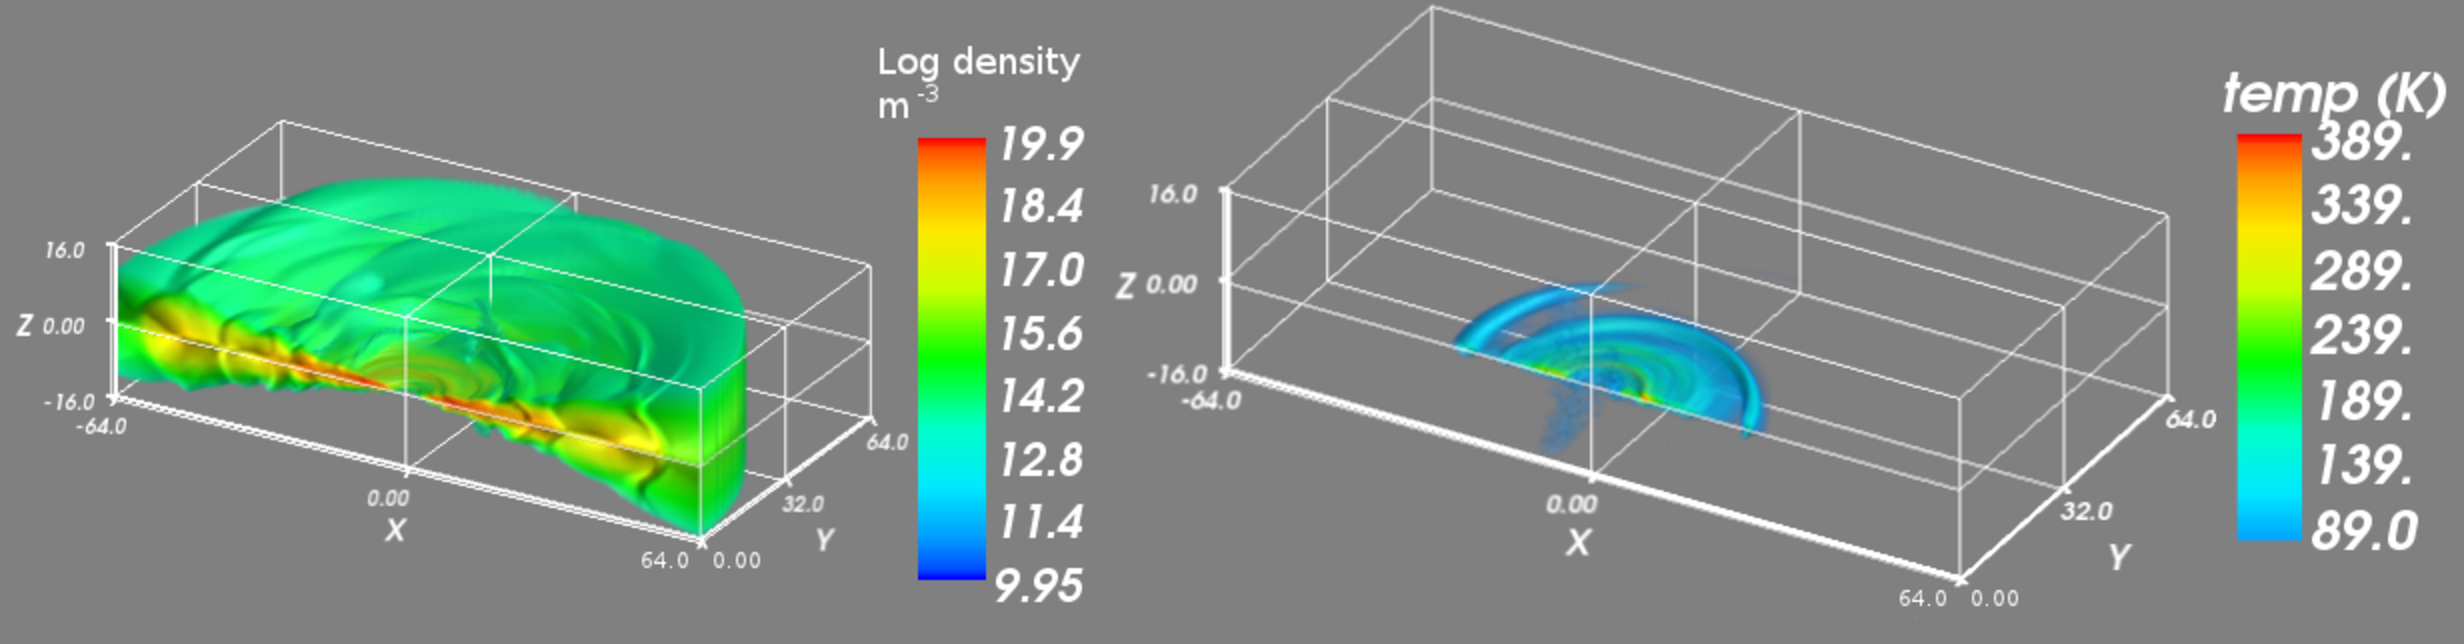
\includegraphics[width=168mm]{Figures/model/rhoT.png}

 \caption{this is a density \& temp plot}
\end{figure*}

\begin{figure*}
 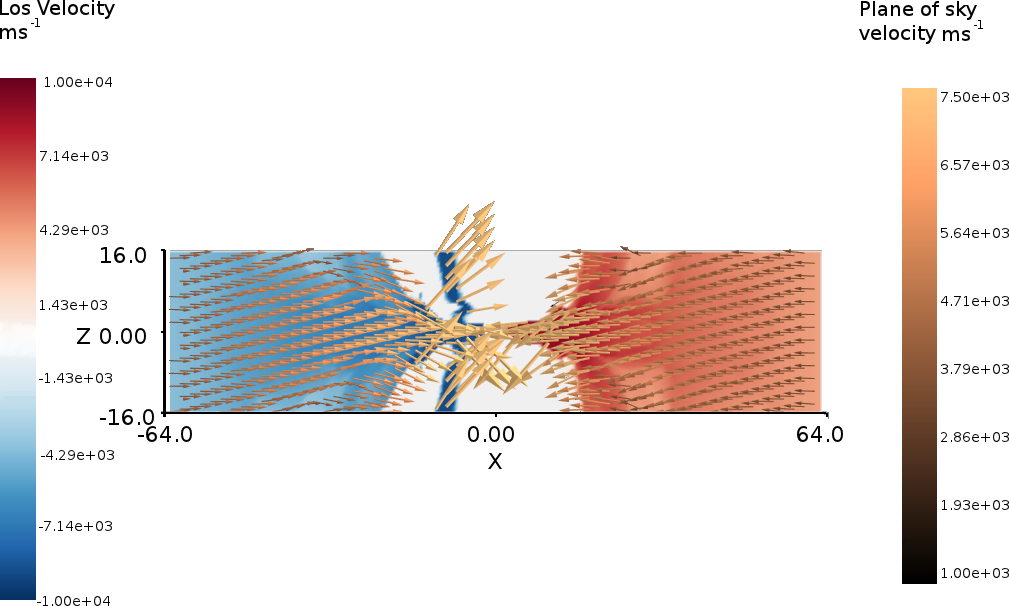
\includegraphics[width=168mm]{Figures/model/velocity_rzSlice_thetaColourScale2.png}

 \caption{this is a velocity slice in the rz plane}
\end{figure*}


-describe the physical structure of the disk (density and temperature) -- one figure showing the physical structure and the kinematics (2-panels figure)
The physical structure of the disc is the same as the one used in Ilee et al. (2011), based on the work of Boley(2007), Boley \& Durisen(2008) and Boley(2009). This model describes a 0.39$\,\rm{M}_\odot$ self-gravitating disc featuring prominent spiral arms. Densities in the disc range from 10$^{10}$-10$^{21}\,\rm{m}^{-3}$, and temperatures range from 30-400 K. The dust and gas temperatures in the disc are assumed to be equal. The gas/dust mass ratio was assumed to be 1/100 throughout the model and the opacities were given by the model of dust grains with thick icy mantles and 10$^6\,$yr coagulation from Ossenkopf and Henning (1994). The model is sampled over a regular grid of size 256$\times$256$\times$64 with spatial resolution of 0.5$\,$au in x, y and z. The majority of the mass lies in the mid-plane of the disc. For the models using a smoothed disc the same physical and chemical model is used but with the temperature, density and abundance averaged in $\phi$.\newline

-describe the chemistry  - refer to Ilee et al. which have been taken as input to the rad transfer (RT) code
Chemical abundances in the disc were taken from Ilee et. al (2011) which followed the changes of chemical abundances of trace particles moving through the disc as it evolved. The abundances of 125 species related by 1334 reactions were followed through the time evolution of the disc. These abundances were interpolated onto a 51$^3$ grid covering the disc with cells of size 2.2$\times$2.2$\times$0.22$\,$au. Abundances in the envelope model were as follows:\newline

(tableify this?)\newline
HCO$^+$: as the H2O profile from (find out where L1544 H2O profile is from) scaled so that the maximum abundance is 10$^{-8}$\newline
HNO: constant abundance of 5$\times$10${-11}$\newline
HCS$^+$: 10$^{-11}$\newline
OCS: constant abundance of 10$^{-9}$\newline
H$_2$CO: 1.5$\times$10$^{-9}$ decreased by a factor of 40 at radii less than 8250au (Young et al 2004)\newline
CS:  3$\times$10$^{-9}$ decreased by a factor of 10,000 at radii less than 6700au (Tafalla, santiago-garcia and myers 2006)\newline
CO: as the H2O profile from ??? scaled so that the maximum abundance is CO maximum\newline\


-describe the RT used (LIME) 
LIME (Brinch 2011), the radiative transfer program used, calculates line intensities based on a weighted sample of randomly chosen points in a continuous 3d model. The method of selecting these points is given in the griding section. At each of these points the density of the main collision partner (in this case H$_2$), gas and dust temperatures, velocity, molecular abundances and turbulent velocity and taken from the model. These points are then smoothed by Lloyds algorithm (Lloyd 1982) in order to minimise the variation in distance between points whilst keeping the same underlying distribution. These points are then connected by Delaunay triangulation and it is down these paths that photons are restricted to propagating. The levels of molecules in question are then  calculated at each of these points from collisional and radiative (de)excitation and the local radiation field is calculated. This is repeated 20 times with the populations of each level converging towards a single value. \newline


\begin{figure}
 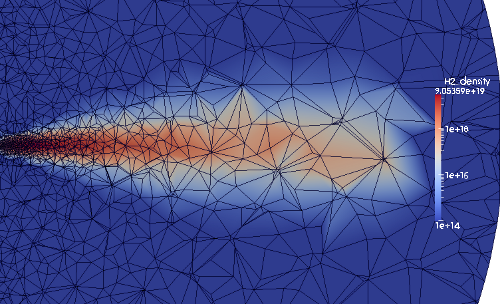
\includegraphics[width=84mm]{Figures/model/Lime_grid3.png}

 \caption{plot of the griding overlaid on a smoothed density model}
\end{figure}

\begin{figure}
 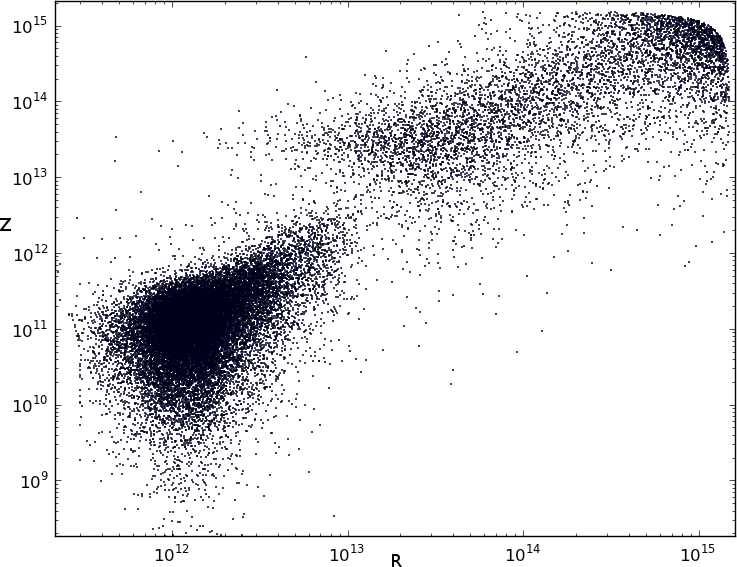
\includegraphics[width=84mm]{Figures/model/lime_points_rz2.png}

 \caption{plot of the points selected in the model}
\end{figure}

In order to construct the grid, points are randomly selected from the volume being simulated then compared against a reference point. Grid points are selected at random in cylindrical co-ordinates, linearly spaced in z and $\phi$ and logarithmically spaced in r. For each point to be selected a random number $\alpha$ is drawn from the semi-open set [0,$\,$1) as a threshold. After selection of random co-ordinates the Hydrogen density and molecular density at the point (n and m) are compared against the densities of a reference point on the inner edge of the disc (n$_0$ and m$_0$). If $\alpha<\left( \frac{n}{n_0} \right)^{0.3}$ or $\alpha< \left( \frac{m}{m_0} \right)^{0.3}$ then the point is selected for use, if not then another r,$\phi$,z co-ordinate is selected. The weighting function and griding functions were selected empirically to sample both the all scales while ensuring the majority of the points went into the inner disc which is the region of interest. 20\% of these points are forced to be at radii greater than $\sqrt{R_{min}R_{max}}$ (where $R_{min}$ and $R_{max}$ are the inner and outer radius of the model) in order to stop too many of the selecected points clustering in the high density disc and leaving the envelope undersampled. In addiation to this method of selection 5\% of the points are linearly distributed in x, y and z with no bias with regards to density or abundance. This provides a minimum level of sampling for the large low density regions in the outer parts of the simulated volume. See figure 5 for example of the points distribution in r, z.


\section{Model Results}

Figures showing the RT results in a few molecules/transitions (CO, HCO$^+$, HCN, OCS, H2CO, NH3 --- maybe H2O,H2$^{18}$O [to try first]) (Note the moment 1 and 0 map were created by integrating between -12.5 to -0.5 km$\,$s$^{-1}$ and +0.5 to +12.5 km$\,$s$^{-1}$ to avoid being dominated by the contribution from the envelope, this can be seen in the some PV diagrams as the strong absorption feature at all positions around zero velocity, mom1maps are shown with a cutoff of 1/1000 of the peak emission/absorption value)\newline

\begin{figure}
 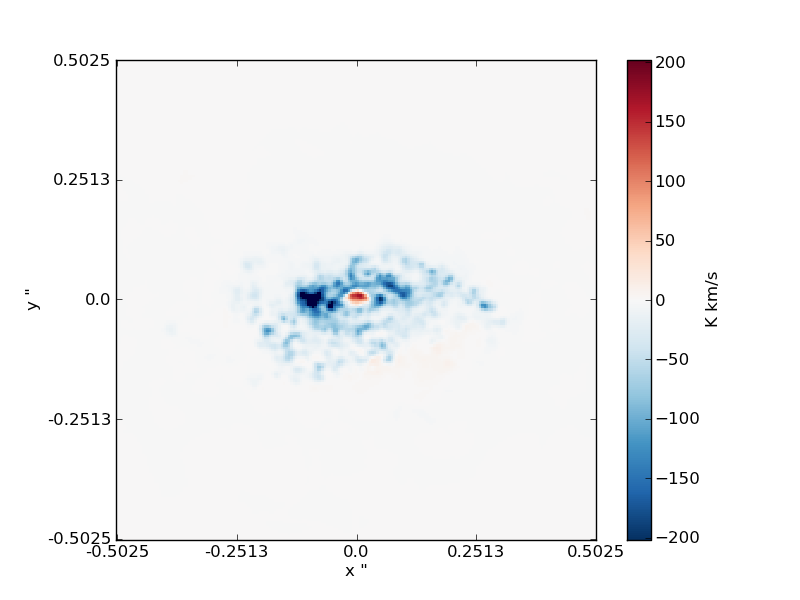
\includegraphics[width=84mm]{Figures/sim/imageCO_3-2_30deg_contSub.png}

 \caption{CO 3-2 Continuum subtracted mom0}
\end{figure}

\begin{figure}
 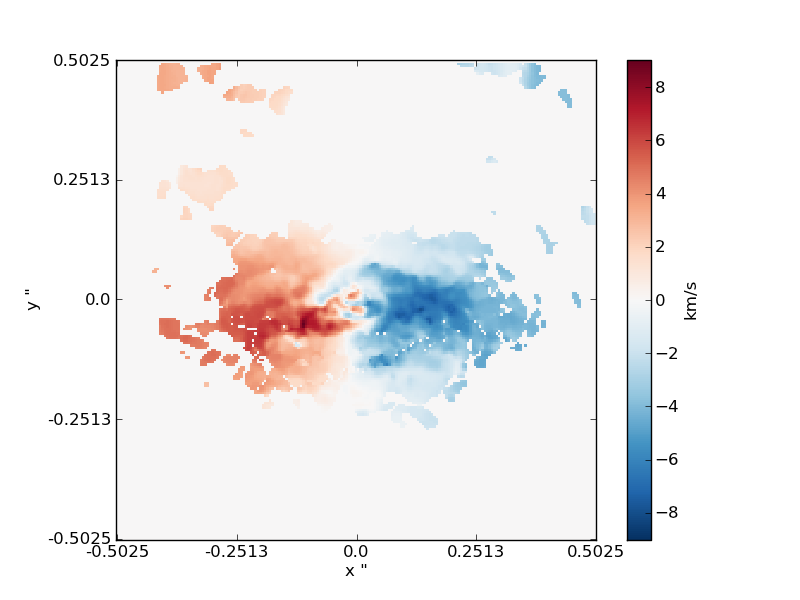
\includegraphics[width=84mm]{Figures/sim/imageCO_3-2_30deg_mom1.png}

 \caption{CO 3-2 mom1map}
\end{figure}

\begin{figure}
 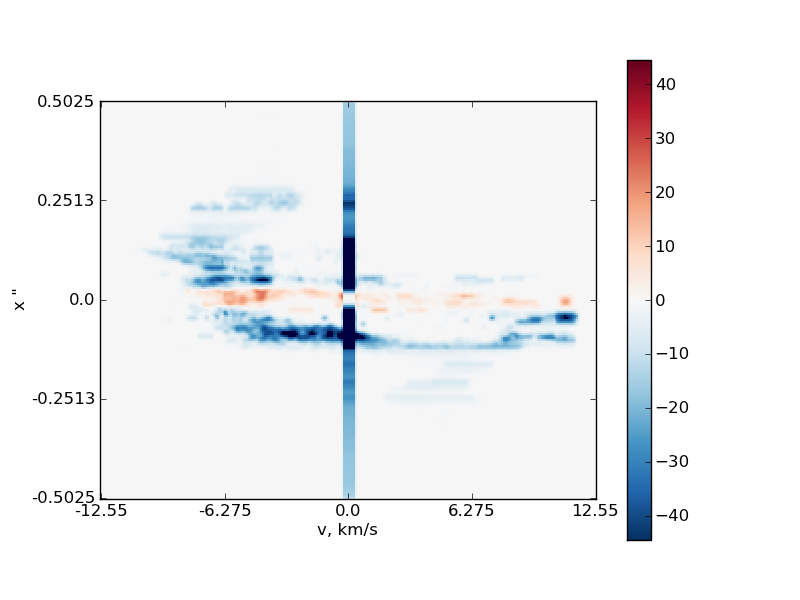
\includegraphics[width=84mm]{Figures/sim/imageCO_3-2_30deg_PV_centre.png}

 \caption{CO 3-2 PV through centre}
\end{figure}

These synthetic images of the CO 3-2 line at 345.8$\,$GHz. As the upper level for this line is at 33$\,$K above the ground state this transition should be excited through out disc. CO line will be thick so this is only mapping the outer regions of the disc. Spiral structure can be seen.\newline



\begin{figure}
 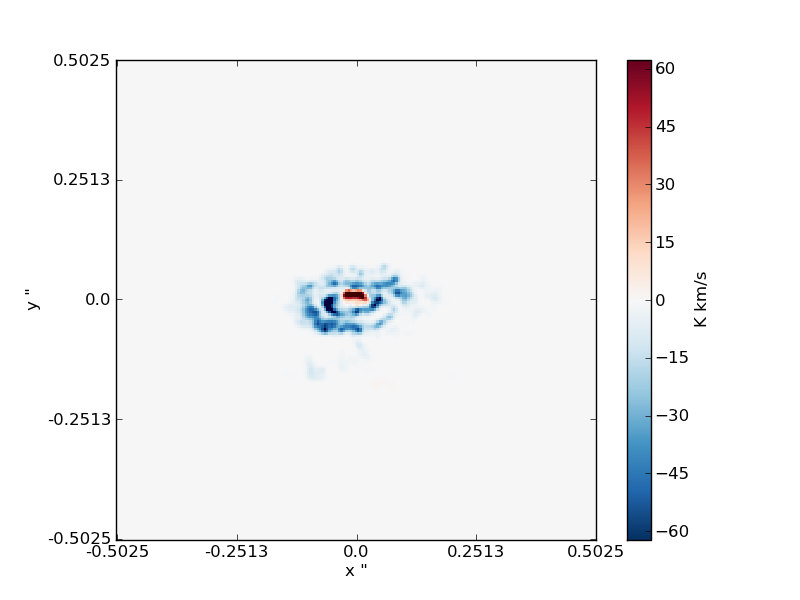
\includegraphics[width=84mm]{Figures/sim/imageOCS_28-27_30deg_contSub.png}

 \caption{OCS 28-27 Continuum subtracted mom0}
\end{figure}

\begin{figure}
 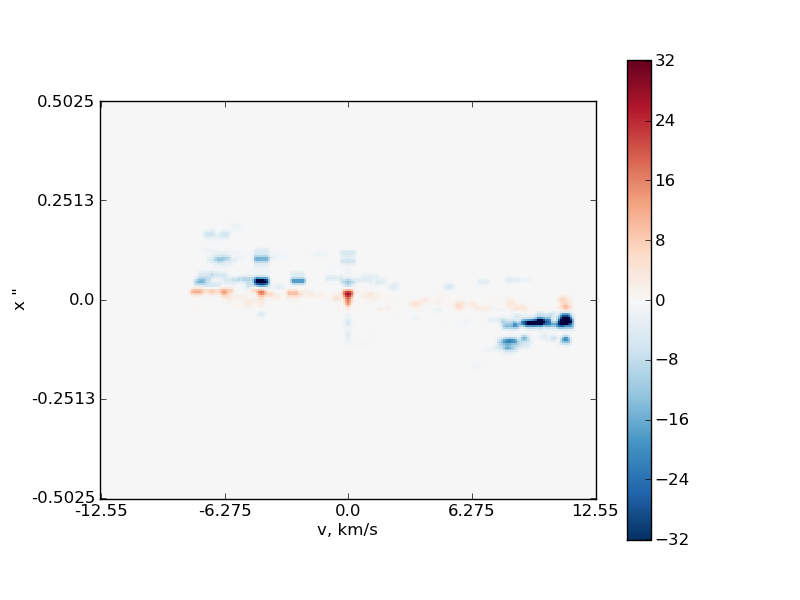
\includegraphics[width=84mm]{Figures/sim/imageOCS_28-27_30deg_PV_centre.png}

 \caption{OCS 28-27 PV through centre}
\end{figure}

The OCS lines in alma band 7 (22-21 through 30-29) with upper energy levels between 161 and 271 K above the ground state provide a way to trace hot shocked gas in spiral arms without resolving structure.\newline

\begin{figure}
 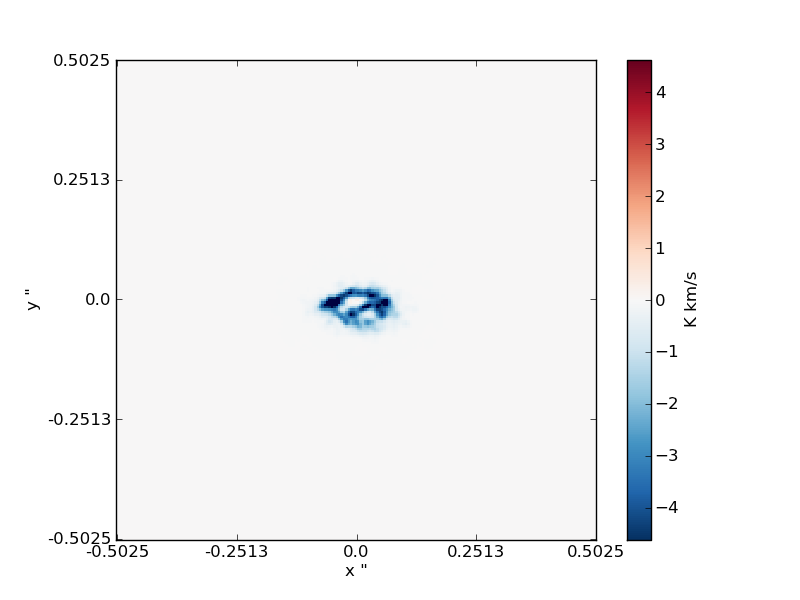
\includegraphics[width=84mm]{Figures/sim/imagesmoothedOCS_28-27_30deg_contSub.png}

 \caption{SmoothedOCS 28-27 Continuum subtracted mom0}
\end{figure}


 
\begin{figure}
 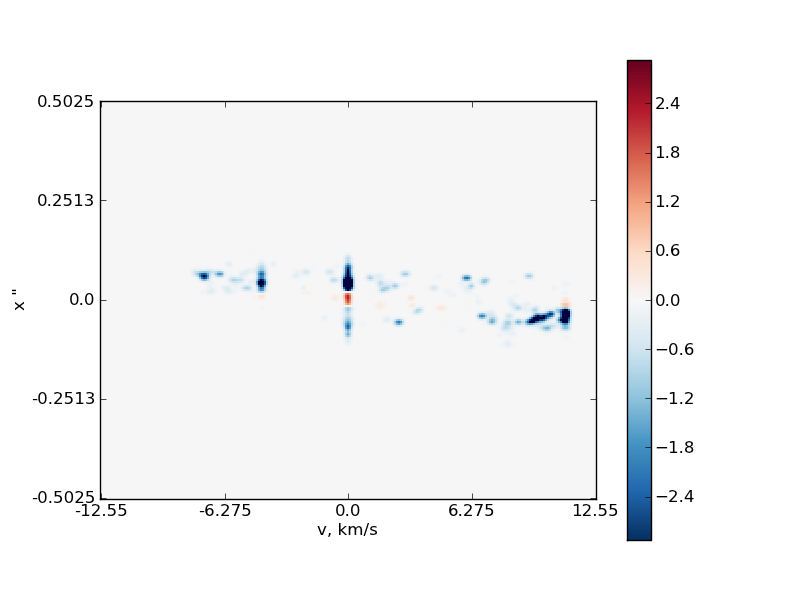
\includegraphics[width=84mm]{Figures/sim/imagesmoothedOCS_28-27_30deg_PV_centre.png}

 \caption{SmoothedOCS 28-27 PV through centre}
\end{figure}

In comparison to the model with spiral arms the absorbtion and emission from this smoothed model is far weaker.\newline

\begin{figure}
 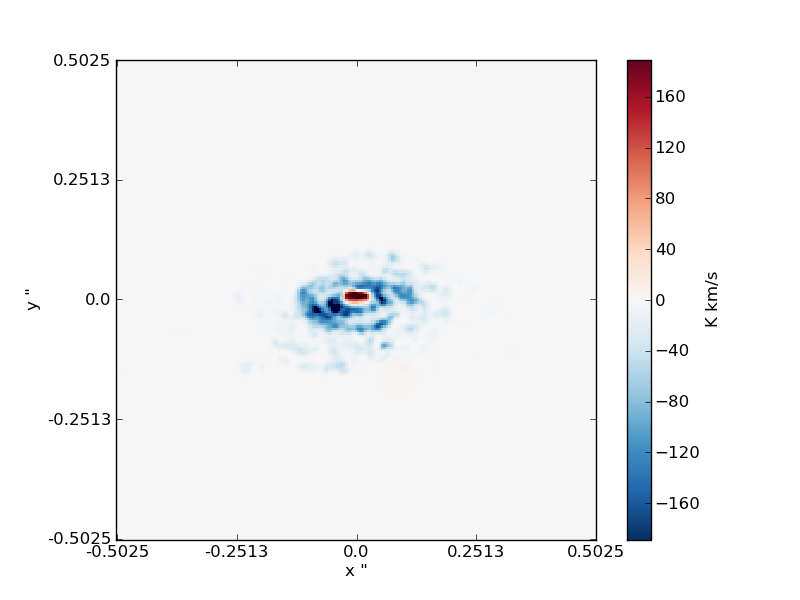
\includegraphics[width=84mm]{Figures/sim/imageH2CO_4-0-4->3-0-3_30deg_contSub.png}

 \caption{H$_2$CO 4$\,$0$\,$4 - 3$\,$0$\,$3 Continuum subtracted mom0}
\end{figure}

\begin{figure}
 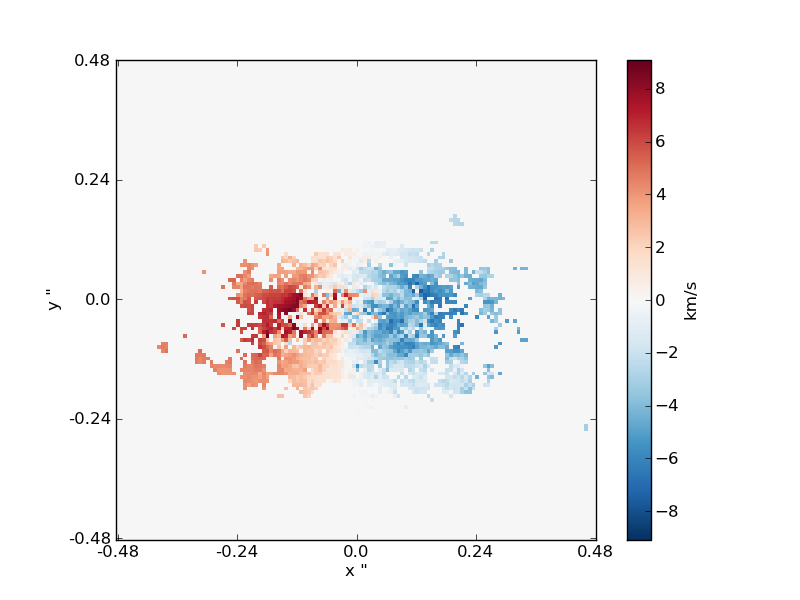
\includegraphics[width=84mm]{Figures/sim/imageH2CO_4-0-4->3-0-3_30deg_mom1.png}

 \caption{H$_2$CO 4$\,$0$\,$4 - 3$\,$0$\,$3 PV through centre}
\end{figure}

\begin{figure}
 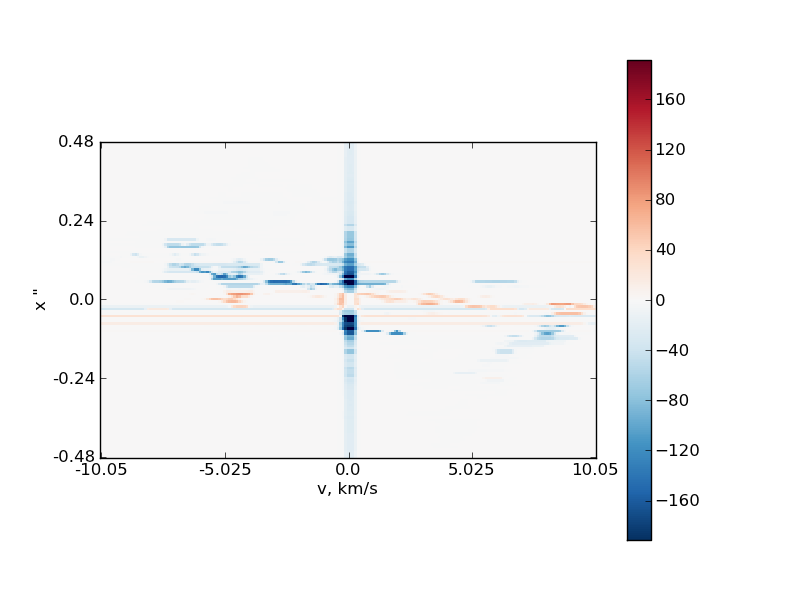
\includegraphics[width=84mm]{Figures/sim/imageH2CO_4-0-4->3-0-3_30deg_PV_centre.png}

 \caption{H$_2$CO 4$\,$0$\,$4 - 3$\,$0$\,$3 PV through centre}
\end{figure}

line ratios of many lined spieces can help us calculate temperatures of the emitting regions.

(figure of temperature as a function of line ratio for 2 sets of formaldehyde lines and map of derived temperature, talk to P about this)\newline

\begin{figure}
 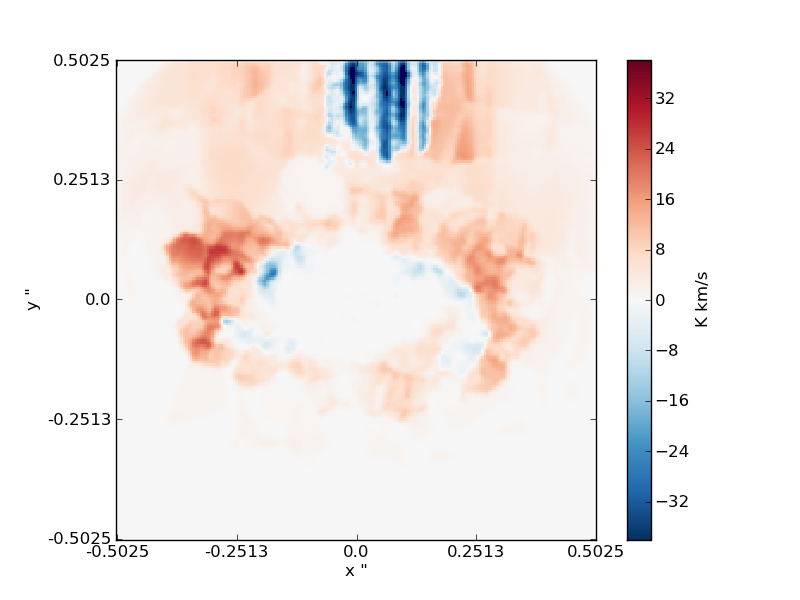
\includegraphics[width=84mm]{Figures/sim/imageHCOp_1-0_30deg_contSub.png}

 \caption{HCO$^+$ 1-0 Continuum subtracted mom0}
\end{figure}

\begin{figure}
 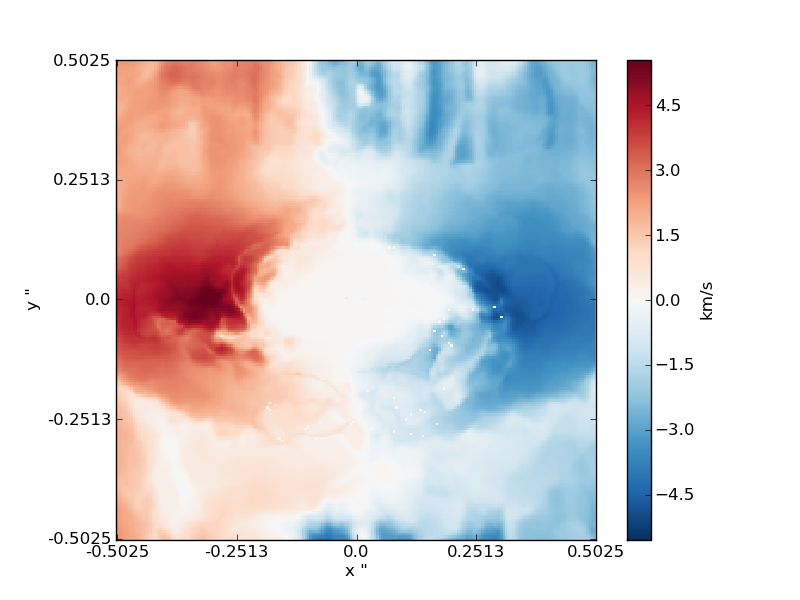
\includegraphics[width=84mm]{Figures/sim/imageHCOp_1-0_30deg_mom1.png}

 \caption{HCO$^+$ 1-0 mom1map}
\end{figure}

\begin{figure}
 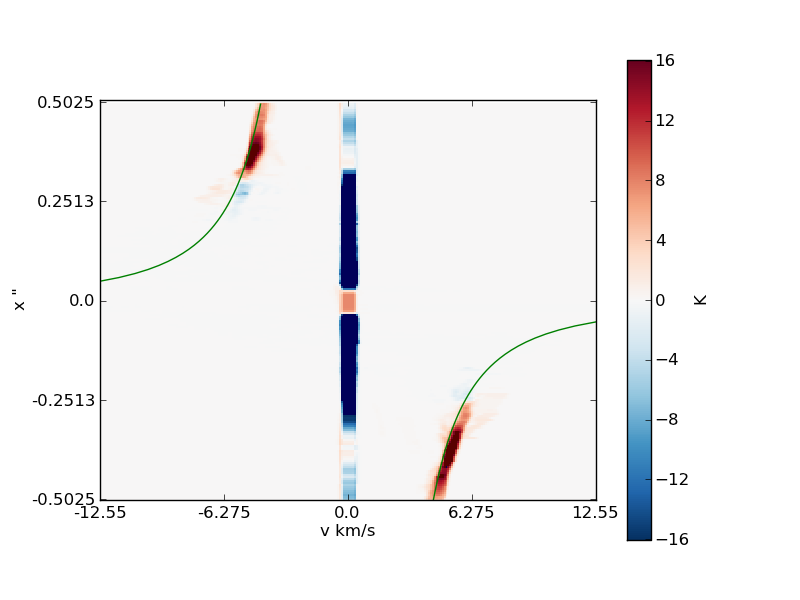
\includegraphics[width=84mm]{Figures/sim/imageHCOp_1-0_30deg_PV_centre.png}

 \caption{HCO$^+$ 1-0 PV through centre}
\end{figure}

some molecules such as HCO$^+$ trace only the inner disc (ref ilee 2011) and so can be used to look at the extended velocity and physical structure.\newline


Figures showing different inclinations  
\begin{figure}
 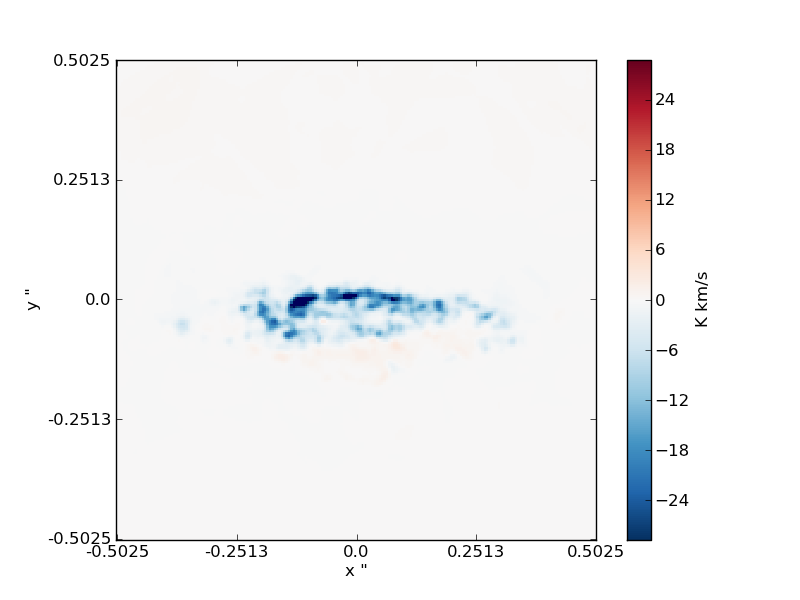
\includegraphics[width=84mm]{Figures/sim/imageC18O_3-2_15deg_contSub.png}

 \caption{C18O 3-2 15 deg Continuum subtracted mom0}
\end{figure}

\begin{figure}
 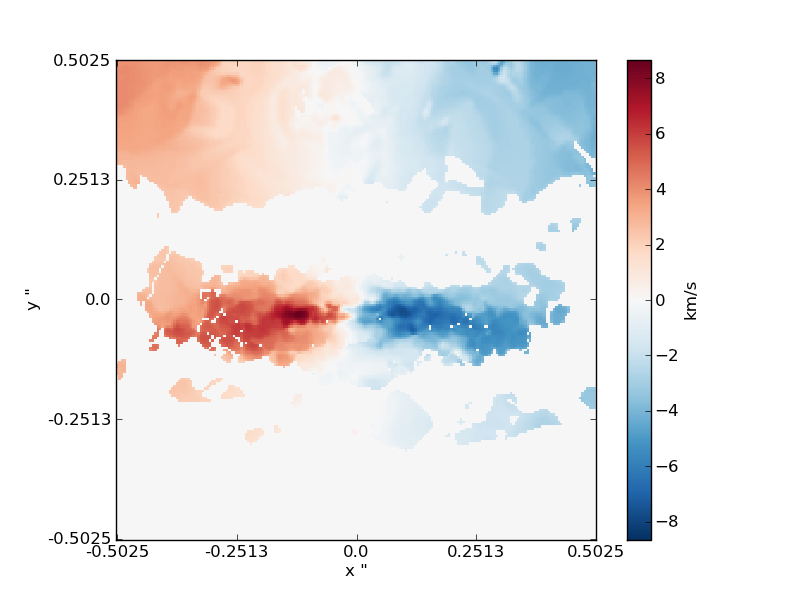
\includegraphics[width=84mm]{Figures/sim/imageC18O_3-2_15deg_mom1.png}

 \caption{C18O 3-2 15 deg mom1map}
\end{figure}

\begin{figure}
 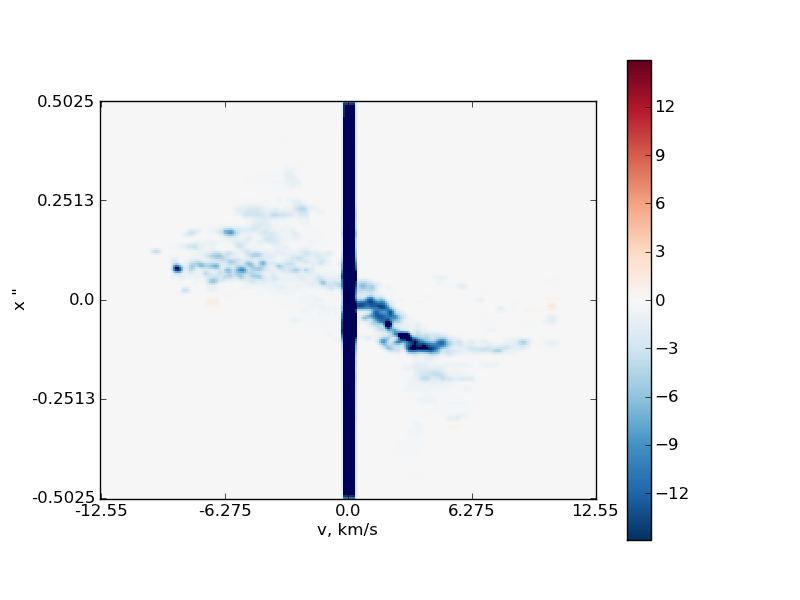
\includegraphics[width=84mm]{Figures/sim/imageC18O_3-2_15deg_PV_centre.png}

 \caption{C18O 3-2 PV 15 deg through centre}
\end{figure}


\begin{figure}
 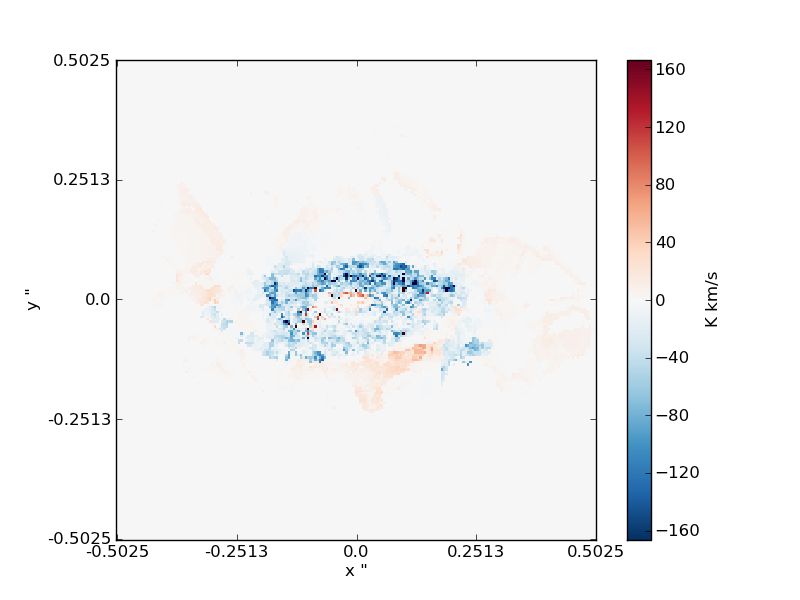
\includegraphics[width=84mm]{Figures/sim/imageC18O_3-2_30deg_contSub.png}

 \caption{C18O 3-2  30 deg Continuum subtracted mom0}
\end{figure}

fdagfdabfdsbfdbds fdbfd  fdfbfvdfd g rbfd fdbfdbc \newline fdagfdabfdsbfdbds fdbfd  fdfbfvdfd g rbfd fdbfdbc \newline fdagfdabfdsbfdbds fdbfd  fdfbfvdfd g rbfd fdbfdbc \newline fdagfdabfdsbfdbds fdbfd  fdfbfvdfd g rbfd fdbfdbc \newline fdagfdabfdsbfdbds fdbfd  fdfbfvdfd g rbfd fdbfdbc \newline fdagfdabfdsbfdbds fdbfd  fdfbfvdfd g rbfd fdbfdbc \newline


\begin{figure}
 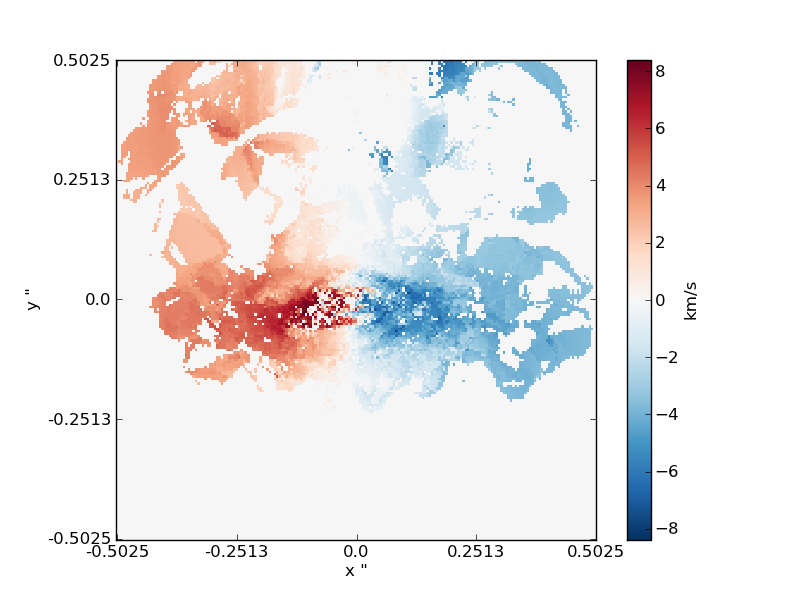
\includegraphics[width=84mm]{Figures/sim/imageC18O_3-2_30deg_mom1.png}

 \caption{C18O 3-2 30 deg mom1map}
\end{figure}

\begin{figure}
 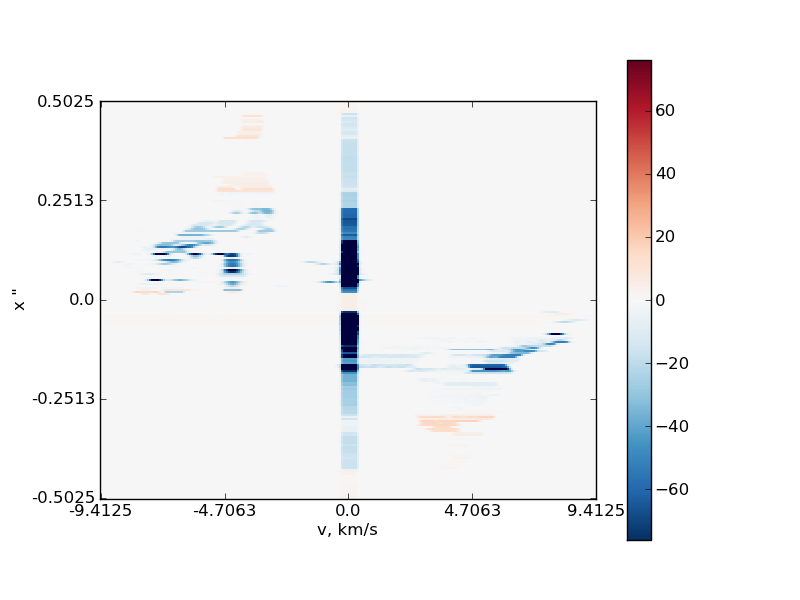
\includegraphics[width=84mm]{Figures/sim/imageC18O_3-2_30deg_PV_centre.png}

 \caption{C18O 3-2 30 deg PV through centre}
\end{figure}

\begin{figure}
 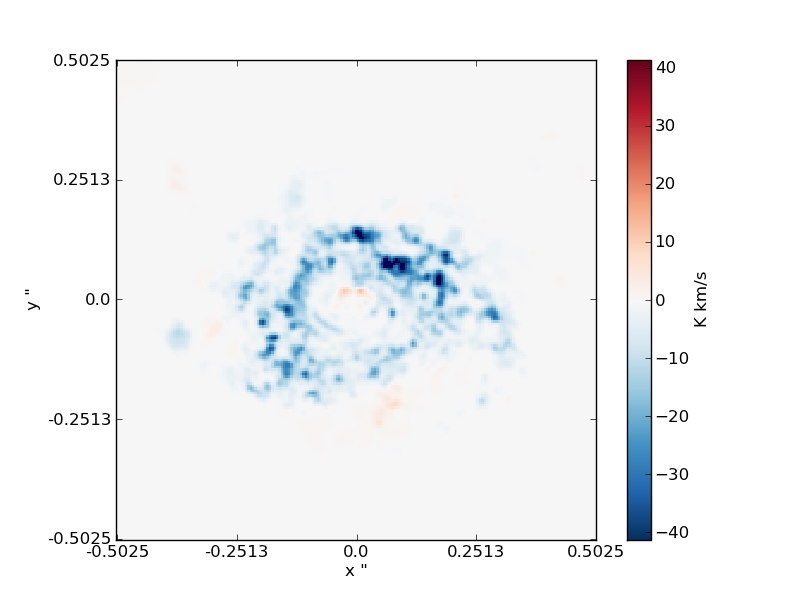
\includegraphics[width=84mm]{Figures/sim/imageC18O_3-2_45deg_contSub.png}

 \caption{C18O 3-2 45 deg Continuum subtracted mom0}
\end{figure}

\begin{figure}
 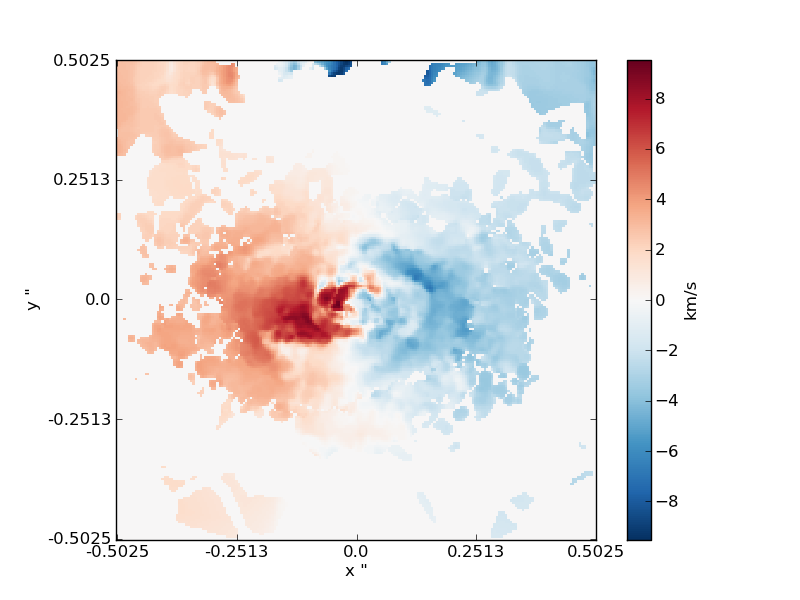
\includegraphics[width=84mm]{Figures/sim/imageC18O_3-2_45deg_mom1.png}

 \caption{C18O 3-2 45 deg mom1map}
\end{figure}

\begin{figure}
 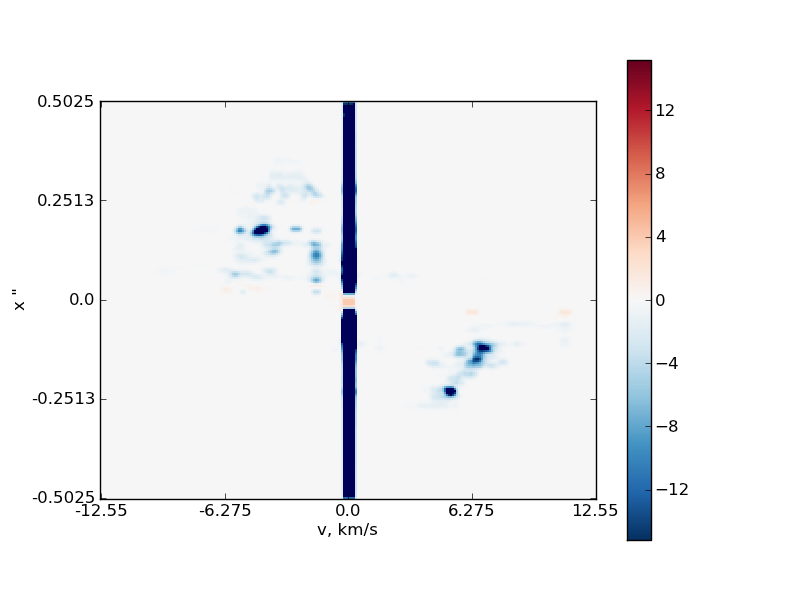
\includegraphics[width=84mm]{Figures/sim/imageC18O_3-2_45deg_PV_centre.png}

 \caption{C18O 3-2 45 deg PV through centre}
\end{figure}

nfsdankjdsankj vdjsk nvjdks nvkds jkkd jkvd jkvf djk fj\newline nfsdankjdsankj vdjsk nvjdks nvkds jkkd jkvd jkvf djk fj\newline nfsdankjdsankj vdjsk nvjdks nvkds jkkd jkvd jkvf djk fj\newline nfsdankjdsankj vdjsk nvjdks nvkds jkkd jkvd jkvf djk fj\newline nfsdankjdsankj vdjsk nvjdks nvkds jkkd jkvd jkvf djk fj\newline nfsdankjdsankj vdjsk nvjdks nvkds jkkd jkvd jkvf djk fj\newline nfsdankjdsankj vdjsk nvjdks nvkds jkkd jkvd jkvf djk fj\newline 

\begin{figure}
 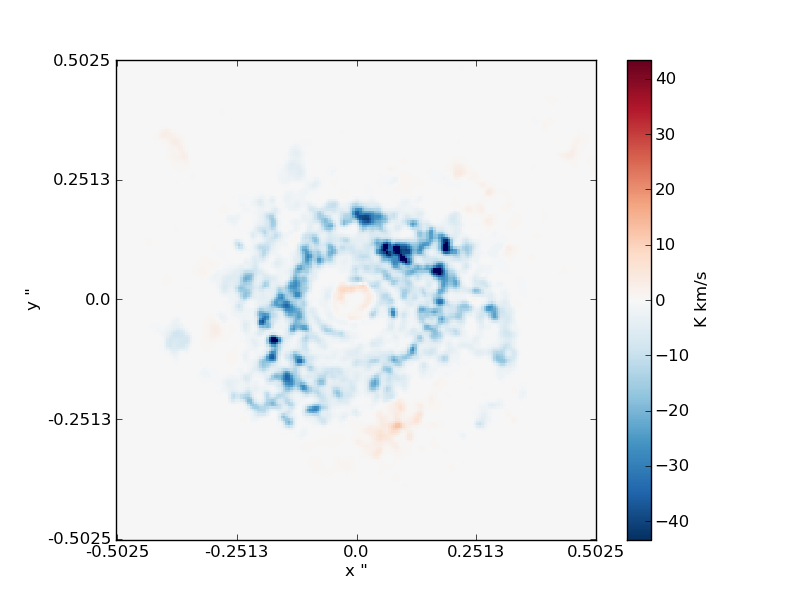
\includegraphics[width=84mm]{Figures/sim/imageC18O_3-2_60deg_contSub.png}

 \caption{C18O 3-2 60 deg Continuum subtracted mom0}
\end{figure}

\begin{figure}
 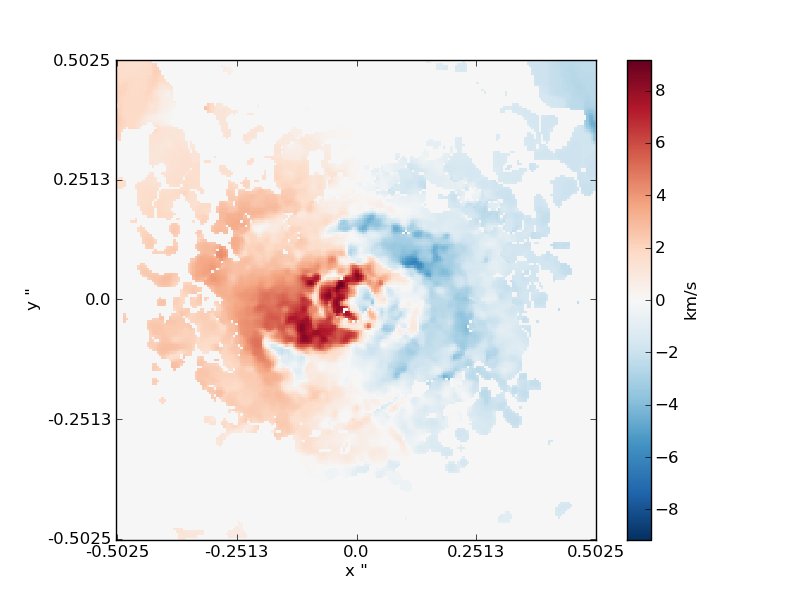
\includegraphics[width=84mm]{Figures/sim/imageC18O_3-2_60deg_mom1.png}

 \caption{C18O 3-2 60 deg mom1map}
\end{figure}

\begin{figure}
 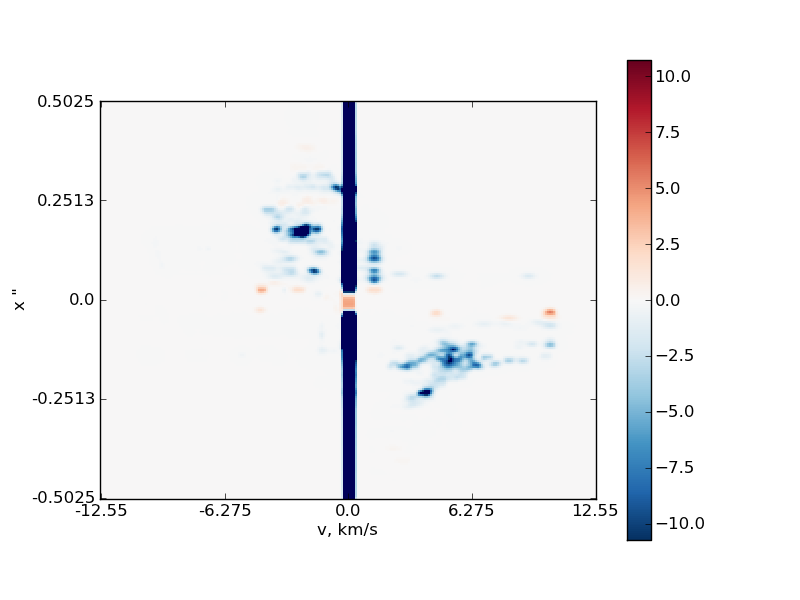
\includegraphics[width=84mm]{Figures/sim/imageC18O_3-2_60deg_PV_centre.png}

 \caption{C18O 3-2 60 deg PV through centre}
\end{figure}

\begin{figure}
 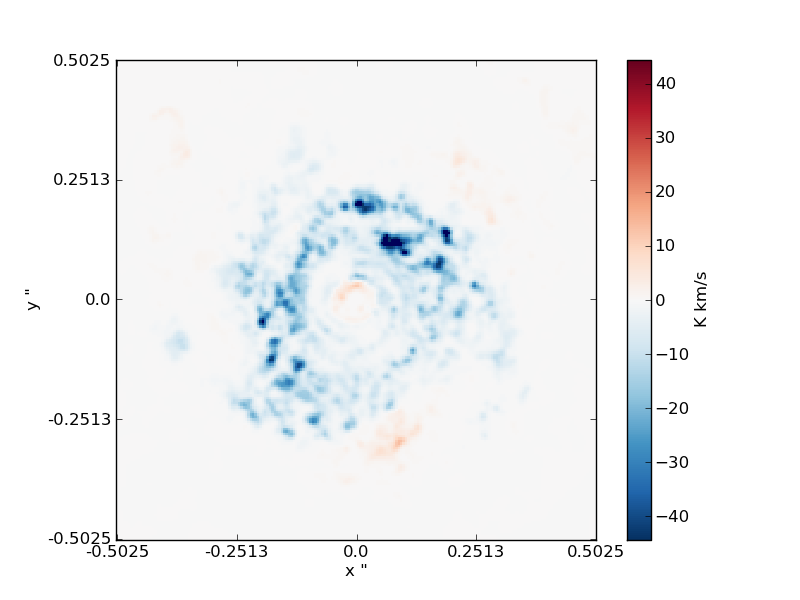
\includegraphics[width=84mm]{Figures/sim/imageC18O_3-2_75deg_contSub.png}

 \caption{C18O 3-2 75 deg Continuum subtracted mom0}
\end{figure}

\begin{figure}
 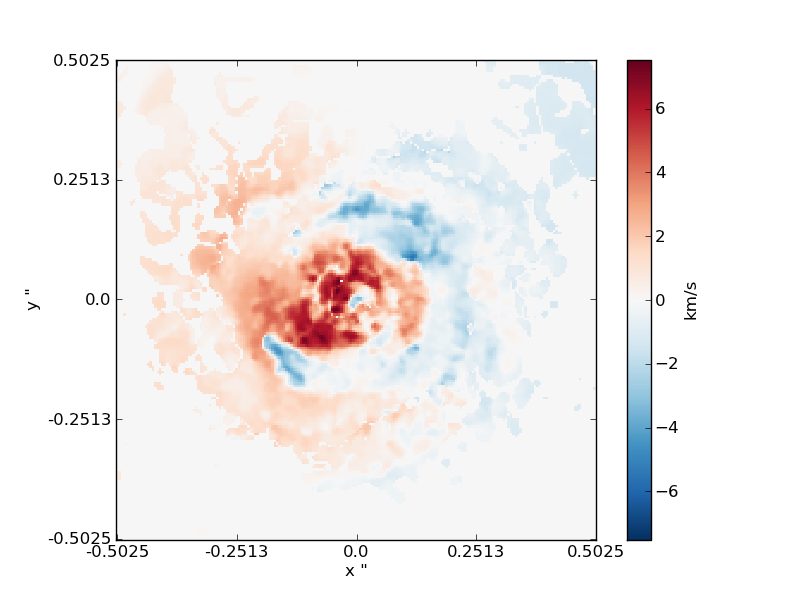
\includegraphics[width=84mm]{Figures/sim/imageC18O_3-2_75deg_mom1.png}

 \caption{C18O 3-2 75 deg mom1map}
\end{figure}

\begin{figure}
 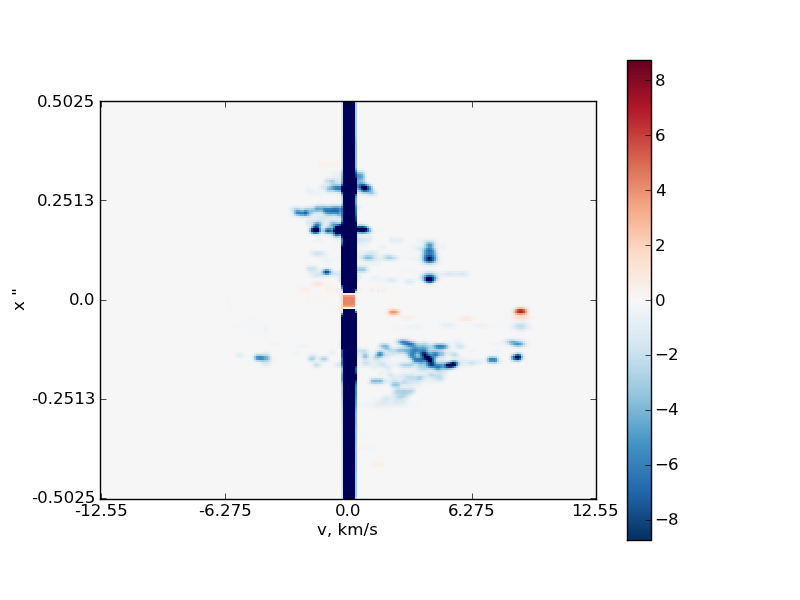
\includegraphics[width=84mm]{Figures/sim/imageC18O_3-2_75deg_PV_centre.png}

 \caption{C18O 3-2 75 deg PV through centre}
\end{figure}


Figure showing different transitions of the same molecule (e.g. CO(1-0), ...(7-6) , OCS,  H2CO ) for same inclination but in different disks (Boley et al. and the smooth disk)\newline

\section{ALMA Predictions}

- current status (Cycle 1) - Figure
OCS + C18O + H2CO + HNO/CS/
- final status - Figure 


\section{Conclusions}

note that all species show up in absorption and some show a little bit of emission around the edges of the disc
OCS is good for showing up spiral structure without being able to resolve it.
envelope only contaminates the central plus-minus 500 m/s or so


\section*{Acknowledgements}

I thank Professor N. Kameswara Rao for some helpful suggestions,
Dr H. C. Bhatt for a critical reading of the original version of the
paper and an anonymous referee for very useful comments that improved
the presentation of the paper.


%\appendix
%
%\section[]{Large gaps in L\lowercase{y}${\balpha}$ forests\\* due to fluctuations in line %distribution}
%
%(This appendix was not part of the original paper by
%A.V.~Raveendran and is included here just for illustrative
%purposes. The references are not relevant to the text of the
%appendix, they are references from the bibliography used to
%illustrate text before and after citations.)
%
%Spectroscopic observations of bright quasars show that the mean
%number density of Ly$\alpha$ forest lines, which satisfy certain
%criteria, evolves like $\rmn{d}N/\rmn{d}z=A(1+z)^\gamma$, where
%$A$ and~$\gamma$ are two constants.  Given the above intrinsic
%line distribution we examine the probability of finding large gaps
%in the Ly$\alpha$ forests.  We concentrate here only on the
%statistics and neglect all observational complications such as the
%line blending effect \citep[see][for example]{b11}.
%
%Suppose we have observed a Ly$\alpha$ forest between redshifts $z_1$
%and~$z_2$ and found $N-1$ lines.  For high-redshift quasars $z_2$~is
%usually the emission redshift $z_{\rmn{em}}$ and $z_1$ is set to
%$(\lambda_{\rmn{Ly}\beta}/\lambda_{\rmn{Ly}\alpha})(1+z_{\rmn{em}})=0.844
%(1+z_{\rmn{em}})$ to avoid contamination by Ly$\beta$ lines.  We
%want to know whether the largest gaps observed in the forest are
%significantly inconsistent with the above line distribution.  To do
%this we introduce a new variable~$x$:
%%
%\begin{equation}
%x={(1+z)^{\gamma+1}-(1+z_1)^{\gamma+1} \over
%     (1+z_2)^{\gamma+1}-(1+z_1)^{\gamma+1}}.
%\end{equation}
%%
%$x$ varies from 0 to 1.  We then have $\rmn{d}N/\rmn{d}x=\lambda$, where $\lambda$
%is the mean number of lines between $z_1$ and $z_2$ and is given by
%%
%\begin{equation}
%\lambda\equiv{A[(1+z_2)^{\gamma+1}-(1+z_1)^{\gamma+1}]\over\gamma+1}.
%\end{equation}
%%
%This means that the Ly$\alpha$ forest lines are uniformly
%distributed in~$x$. The probability of finding $N-1$ lines between $z_1$
%and~$z_2$, $P_{N-1}$, is assumed to be the Poisson distribution.
%%
%\newpage
%%
%\begin{figure}
%\vspace{11pc}
%\caption{$P(>x_{\rmn{gap}})$ as a function of $x_{\rmn{gap}}$ for,
% from left to right, $N=160$, 150, 140, 110, 100, 90, 50, 45 and~40.
% Compare this with \protect\citet{b15}.}
%\label{appenfig}
%\end{figure}
%
%\subsection{Subsection title}
%
%We plot in Fig.~\ref{appenfig} $P(>x_{\rmn{gap}})$ for several $N$
%values. We see that, for $N=100$ and $x_{\rmn{gap}}=0.06$,
%$P(>0.06)\approx20$ per cent.  This means that the probability of
%finding a gap with a size larger than six times the mean
%separation is not significantly small. When the mean number of
%lines is large, $\lambda\sim N>>1$, our $P(>x_{\rmn{gap}})$
%approaches the result obtained by \citet[fig. 4]{b22} for small
%(but still very large if measured in units of the mean separation)
%$x_{\rmn{gap}}$, i.e., $P(>x_{\rmn{gap}})\sim N(1-
%x_{\rmn{gap}})^{N-1}\sim N {\rmn{exp}}(-\lambda x_{\rmn{gap}})$.
%
\bsp
%
\label{lastpage}
%
\end{document}
